\section{Module}
\label{subs:module}
Since a configuration is made up of individual modules, it seems natural to model it as a set of synchronizing module instances. In this section we will first show off the initial design of the module template. Then discuss how we got more concrete with the final version. 

\subsection{Early module template}
In our early design work we tried to implement most everything brought up in \cref{sec:runningexample}. A module has an identifying name and it may only work on one item at a time. It also takes a certain amount of time to perform each work type and to transport items across modules. However we model modules to only perform one type of work. There are also no physical restrictions on which modules may be connected, other than the fact that a module may not be connected to more than four other modules. These basic ideas turned into our first version of the module template, which can be seen in \cref{fig:earlymodule}.


\begin{figure}[h]
\centering
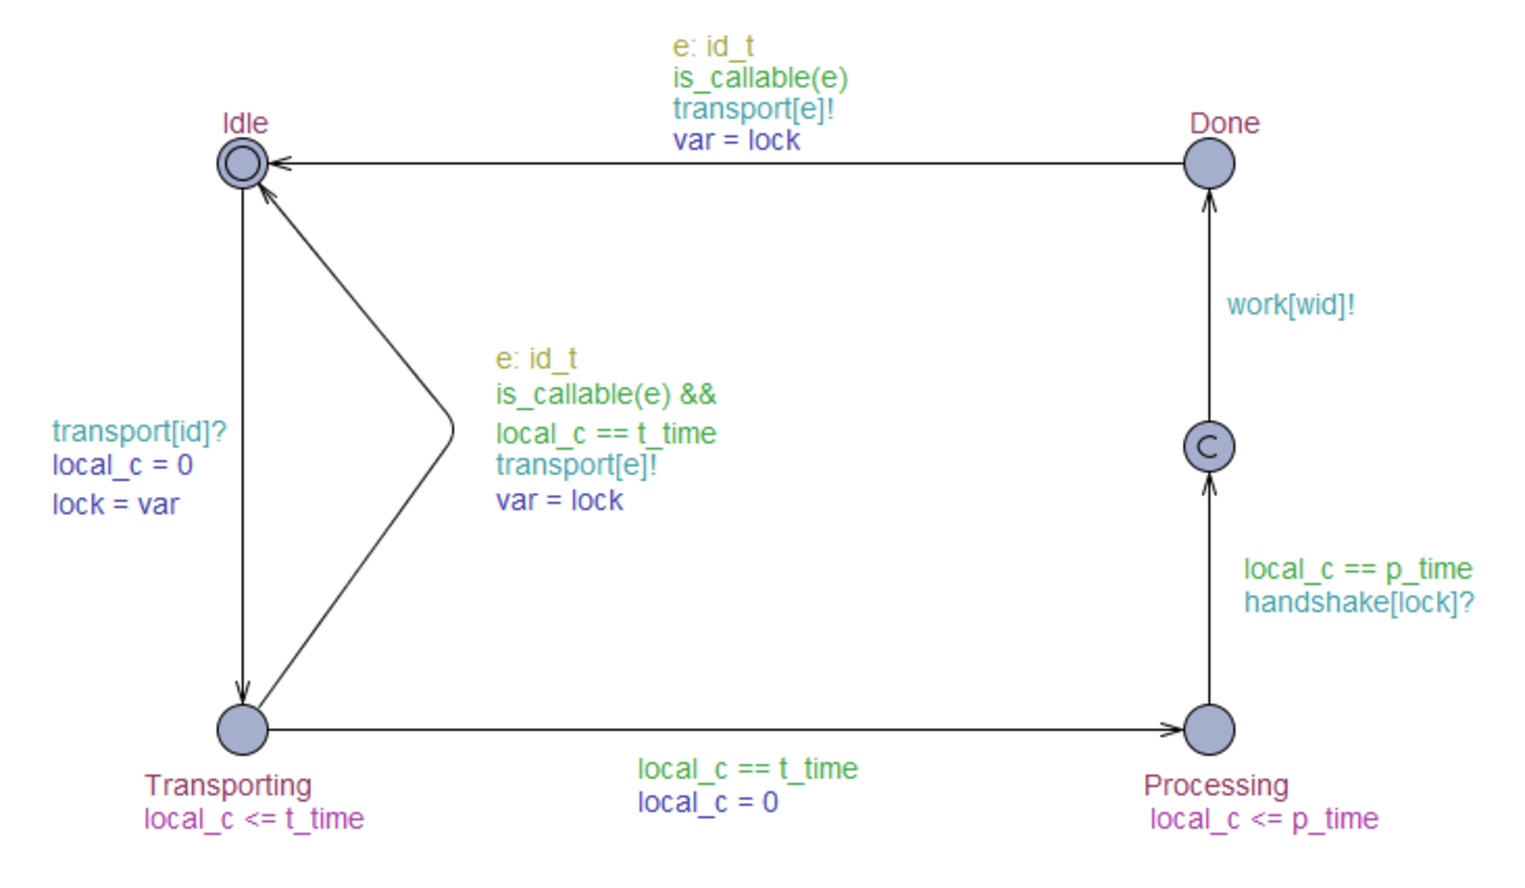
\includegraphics[width=\textwidth]{earlymodule.pdf}
\caption{Early version of the module template}
\label{fig:earlymodule}
\end{figure}

A module resides in the \emph{Idle} location when not processing a recipe. It leaves this location, when one of its up to four neighbouring modules passes on a recipe by synchronizing on the \emph{transport} channel. Once a recipe has been received, the module waits in the \emph{transporting} location for \emph{t\_time}. This simulates the time taken to transport the recipe across the module. Once the time has passed we may send the recipe to a neighbouring module. The guarding function \emph{is\_callable} makes sure, we only send to neighbours. This allows us to implement modules, which are only used for transporting recipes.

Instead of passing the recipe along, we may perform work on it by moving into the \emph{Processing} location. Here we wait for \emph{p\_time}, to simulate the time it takes to work the recipe. Before we can update the recipe to have its work performed, it must identify itself. This is done by synchronizing on the \emph{handshake} channel given by the value stored in the local \emph{lock} variable. The variable contains the unique id of the recipe, which most recently entered the module. It was received from the previous module over the global \emph{var} variable. This ensures that after a handshake, moving us to a committed location, the synchronizing on the \emph{work} channel will be with the correct recipe. Once work has been performed we may pass the recipe onto another module. 

Some modules may also allow for recipes to be removed from the system by transporting on the reserved \emph{transport[0]} channel. No actual module has the id 0. Instead an instance of the \emph{Remover} template is constantly calling on the \emph{transport[0]} channel. If synchronizing is established it does nothing with the received recipe. A module can only synchronize with the remover instance, if it has one of its neighbouring modules set to 0. 

\subsection{Final module template}
From further observations of the local FESTO set-up, we conclude that the above implementation is too abstract. In an actual factory, each module may perform several different types of work on an item, as stated earlier. While only one item is worked at a time, several items may queue up on the module, waiting to be worked on or pass through. A module has a fixed limit of items which may queue up. This is accordance with the safety property of the system. If this is not upheld, items may fly off the modules or the modules themselves may be damaged. Some modules do not allow for items to pass through them, while they are working on another recipe. This feature is not enforced in the above implementation. In addition the time to transport a recipe across a module depend  on the dimensions of the module as well as the directions from which a recipe enters and leaves.

These features lead to some drastic changes in the module template. The biggest is that the template now gets split into three. \emph{ModuleQueue}, which controls the en-queuing and dequeuing of recipes. Then \emph{ModuleWorker} which performs work upon a recipe. Finally \emph{ModuleTransporter}, which transports recipes between modules. To get a complete module, we need an instance of each of these templates sharing the same module id. In the following we will explain each of these new templates.

One aspect that we ultimately do not try to model in UPPAAL are the more extensive physical rules for placing down modules. We choose to enforce these later when generating and comparing configurations. 

\subsubsection{ModuleQueue}\label{subs:modulequeue}
One of the most important characteristics observed was the queuing nature of the system. Several recipes may be located on a module, but only one is being processed at a time. Some of the recipes queued may need to be processed, others just want to be passed along to a neighbouring module. Based on this behaviour we construct the \emph{ModuleQueue} template, which can be seen on \cref{fig:modulequeue}. An instance of this template has a fixed size of modules, which it may hold. Other modules may be able to use the \emph{enqueue} channel to move a recipe onto the module. In addition, recipe may be removed from it through a synchronization on its \emph{dequeue} channel.

As in the earlier version, an item is moved between instances by proxy of its id. The id is always stored in the local \emph{lock} variable.   

\begin{figure}[h]
\centering
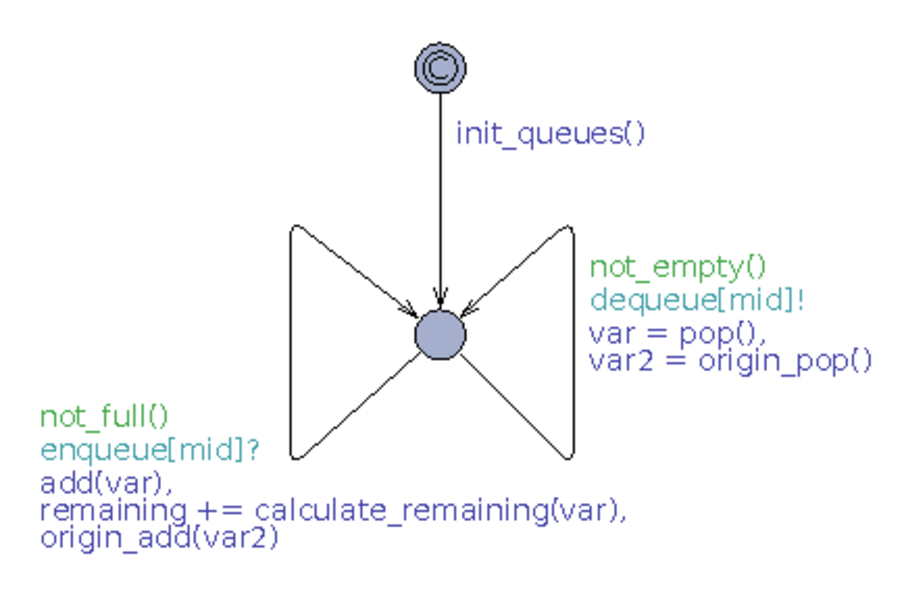
\includegraphics[width=\textwidth]{modulequeue.pdf}
\caption{The ModuleQueue template}
\label{fig:modulequeue}
\end{figure}


\subsubsection{ModuleWorker}\label{subs:moduleworker}
The \emph{ModuleWorker} template can be seen in \cref{fig:moduleworker}. An instance of this template may apply several different types of work upon a recipe. In the idle location, the worker waits to synchronize with the module's \emph{ModuleQueue} instance. If the module can perform some work, it will move into the \emph{Working} location. Here it will wait for \emph{p\_time}, symbolising the time it takes to perform the work. When the wait is over, it will try to synchronize with the recipe through the \emph{handshake} and \emph{work} channels as in the earlier version. Arriving at the \emph{Done} \todo{Maybe call this location something other than Done. In general get names on all the locations} location, we may choose to work the recipe further if possible. Otherwise we perform a synchronization on the module's \emph{intern} channel. This passes the item over to the module's \emph{ModuleTransporter} instance. Synchronization on the intern channel may also occur, if the module cannot perform any work on the recipe. This models the case where an item has to pass through a module without having worked performed, while the model does not allow for pass through while working on other items.

\begin{figure}[h]
\centering
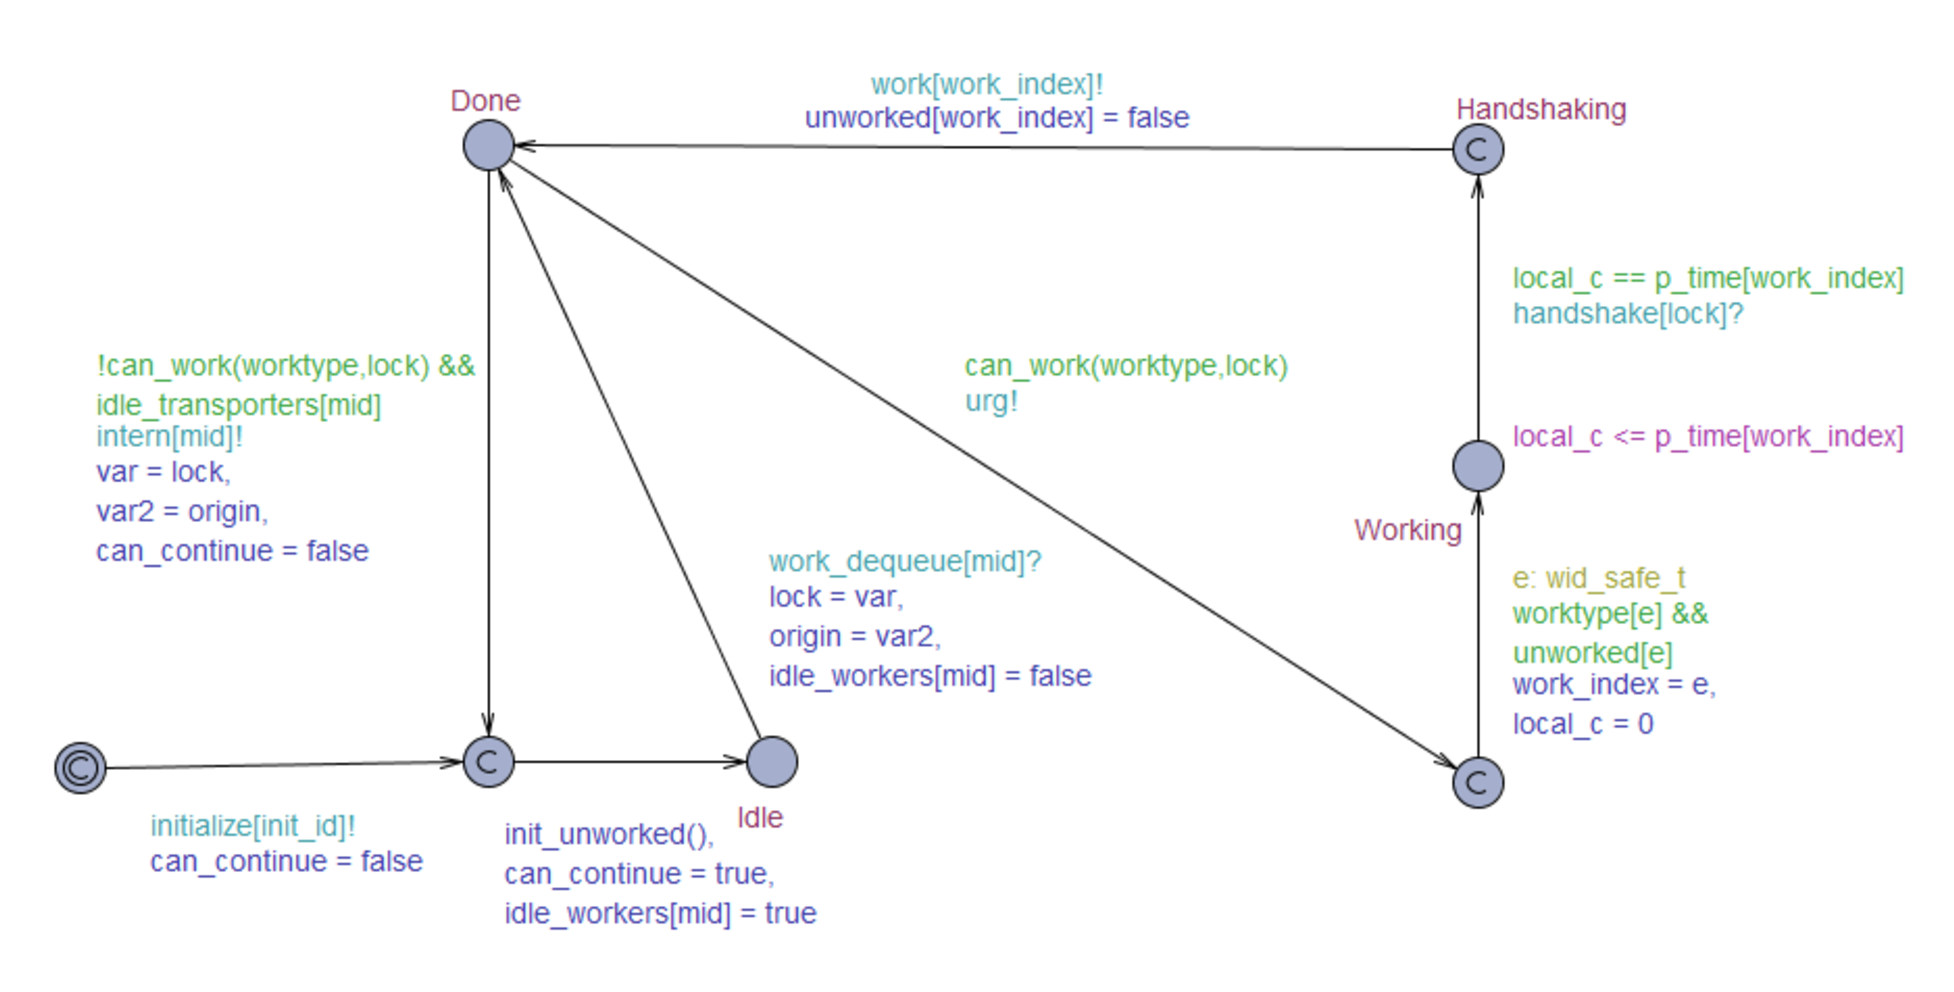
\includegraphics[width=\textwidth]{moduleworker.pdf}
\caption{The ModuleWorker template}
\label{fig:moduleworker}
\end{figure}

\subsubsection{ModuleTransporter}
The \emph{ModuleTransporter} template can be seen in \cref{fig:moduletransporter}. Using an instance of this template, a module may transport an item onto a neighbouring module. If the item comes from the module's \emph{ModuleWorker} instance, then we move into the \emph{Selector} location by synchronizing on the module's \emph{intern} channel. We may however also move directly to the \emph{Selector} location by synchronizing with the module's \emph{ModuleQueue} instance over the \emph{dequeue} channel. This can however only be done, if the \cref{fig:moduletransporter} module allows us to pass a recipe through a module, while it is working on another recipe. This is indicated by the boolean \emph{pass\_through} variable, which is given at instantiation. To create a module only used for transportation, we set this variable to \emph{true} and do not create a \emph{ModuleWorker} instance for the module. 

Once in the \emph{Selector} location a recipe may go to \emph{Idle} or \emph{Transporting}. If the recipe is done, it has to go back to idle and be removed from the production line by synchronizing on the \emph{remove} channel, as opposed to the \emph{transport[0]} in the earlier version.

If the recipe is not done, it may look for a neighbouring module to be passed onto. A module may have up to four neighbours, one on each side. These are stored in the local \emph{next} array, their index indicating their placement relative to the module. When moving to \emph{Transporting} location, the recipe will choose a possible neighbour. In \emph{Transporting} we wait to simulate the time taken to transport a recipe over the module. This time varies according to where the recipe enters the module, and where it leaves. The different transport times are stored in the 4 by 4 multidimensional \emph{t\_time} array. Given that we at this point know the direction, which the recipe entered from \emph{origin} and the direction on which it will leave \emph{succ}, we can look up the exact time to wait in \emph{t\_time}. By implementing this feature we ensure that the time take to pass over a module becomes more accurate to how an item may actually be transported over a module. 

Once the wait is over we move to the \emph{Queuing} location. If the neighbour's queue is full, we wait here until there is room. When possible we synchronize with the neighbours instance of \emph{ModuleQueue} using the \emph{enqueue} channel. At the same time we use the local \emph{inverse} function to calculate, from which side the recipe enters the neighbouring module. This is sent with the global \emph{var2} variable and is later saved into the neighbour's \emph{origin} variable. 

\begin{figure}[h]
\centering
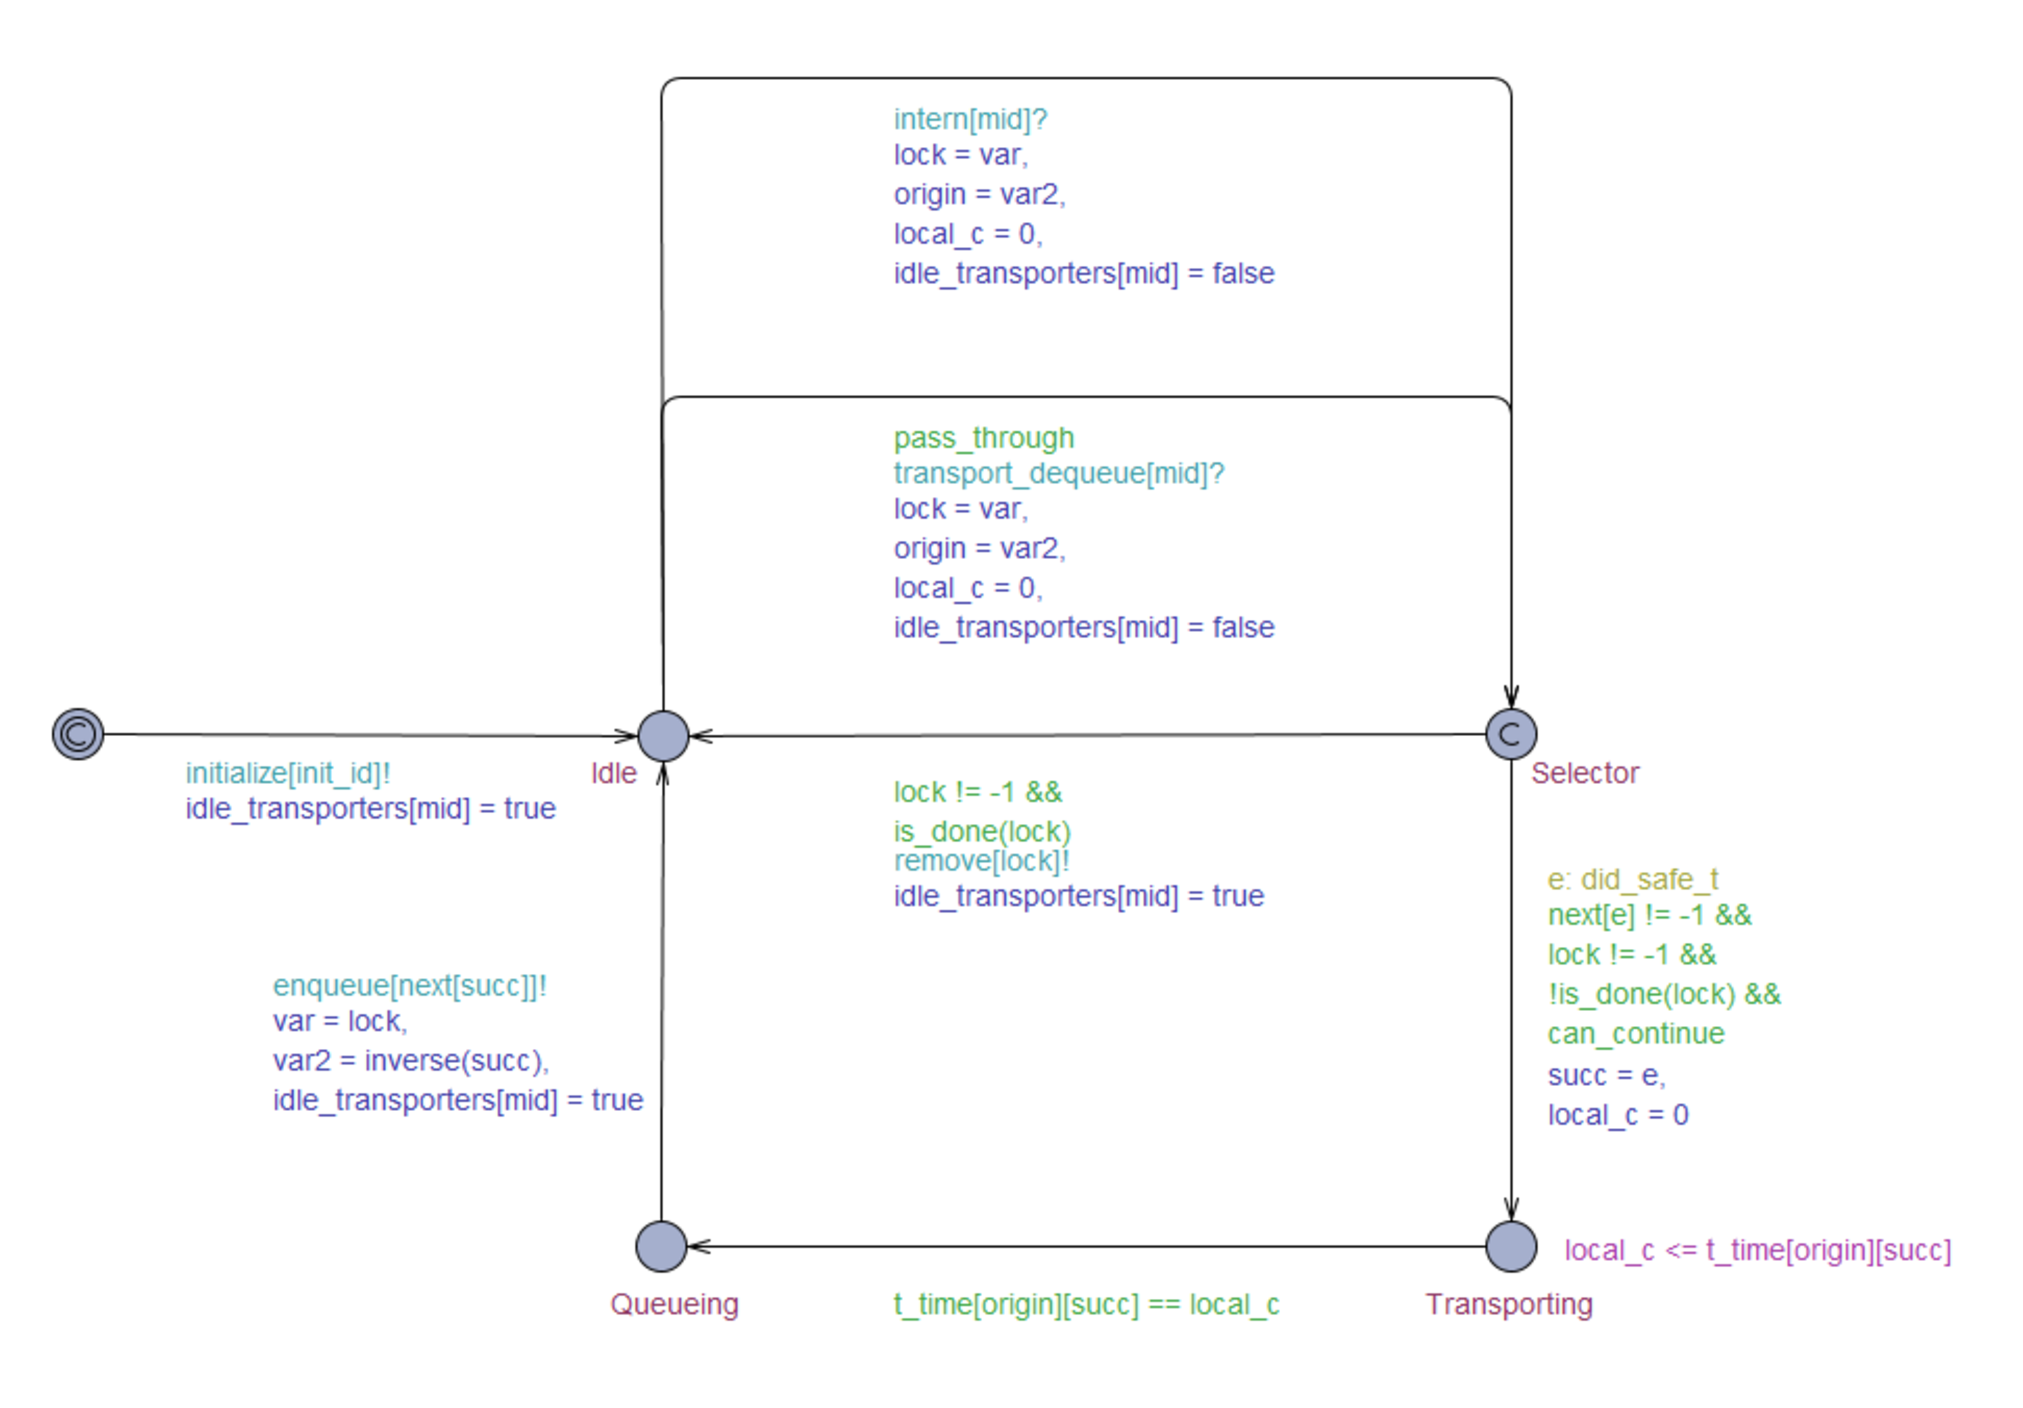
\includegraphics[width=\textwidth]{moduletransporter.pdf}
\caption{The ModuleTransporter template}
\label{fig:moduletransporter}
\end{figure}


